\chapter{Do que as coisas são feitas}\label{ch:g1:materials-around-us}

Olhe uma mesa de café da manhã. Tem uma colher, um copo de leite, um
garfo, um guardanapo, uma tigela e uma blusa de lã pendurada no encosto
da cadeira. São muitas coisas, e cada uma é feita de alguma coisa: a
colher de madeira, o garfo de metal, o copo de vidro, o guardanapo de
papel, a tigela de plástico, a blusa de lã. Uma mesa cheia de coisas,
feitas de só um punhado de materiais diferentes. Este capítulo fala
desses materiais.

\begin{omfigure}
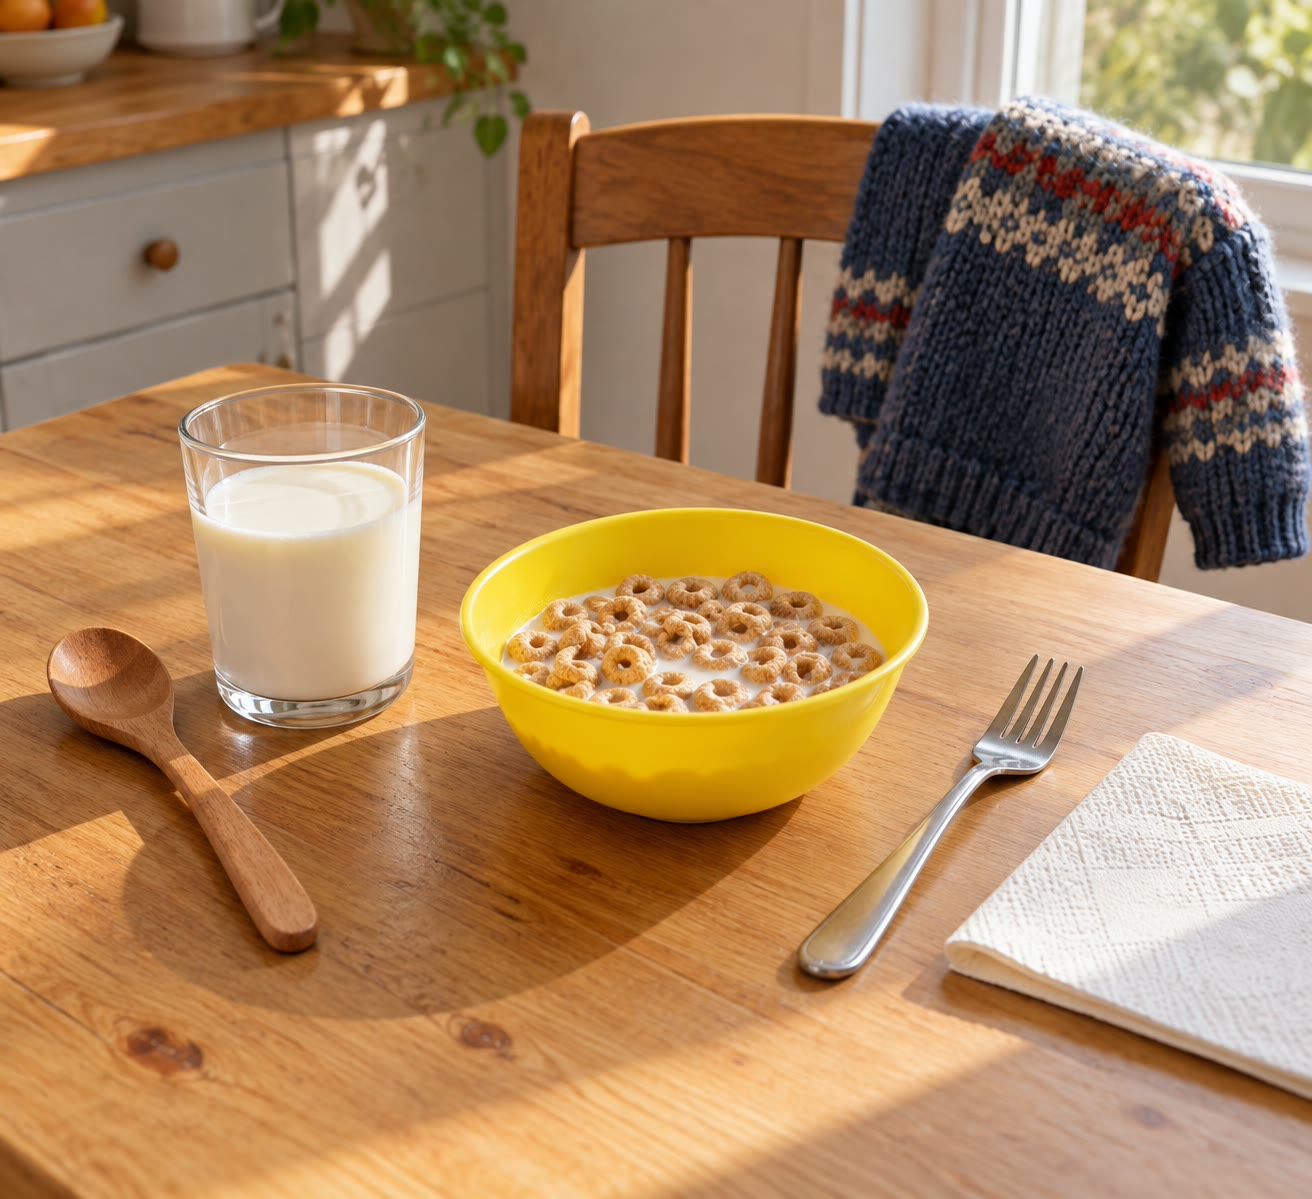
\includegraphics[width=0.62\linewidth]{images/book1/ai/g1-breakfast-table.jpg}

{\small Uma mesa de café da manhã: muitos \omterm{def:g1:materials-around-us:object}{objetos}, feitos de poucos materiais.}
\end{omfigure}

\section{Objetos e materiais}

\begin{definition}[Objeto]\label{def:g1:materials-around-us:object}
Um \emph{objeto}\index{objeto} é uma coisa que podemos ver e tocar, e
muitas vezes segurar e usar: uma colher, uma cadeira, uma bola, uma
janela, um sapato.
\end{definition}

\begin{definition}[Material]\label{def:g1:materials-around-us:material}
O \emph{material}\index{material} de um \omterm{def:g1:materials-around-us:object}{objeto} é aquilo de que o \omterm{def:g1:materials-around-us:object}{objeto}
é feito. Uma colher pode ser feita de madeira, de metal ou de plástico:
a colher é o \omterm{def:g1:materials-around-us:object}{objeto}, a madeira é o material.
\end{definition}

\begin{example}[Um objeto, três materiais]\label{ex:g1:materials-around-us:spoons}
Três colheres estão lado a lado. Elas têm a mesma forma e servem para
a mesma coisa, então são o mesmo tipo de \omterm{def:g1:materials-around-us:object}{objeto}. Mas uma é de madeira,
uma de metal e uma de plástico: três materiais diferentes.
\end{example}

\begin{omfigure}
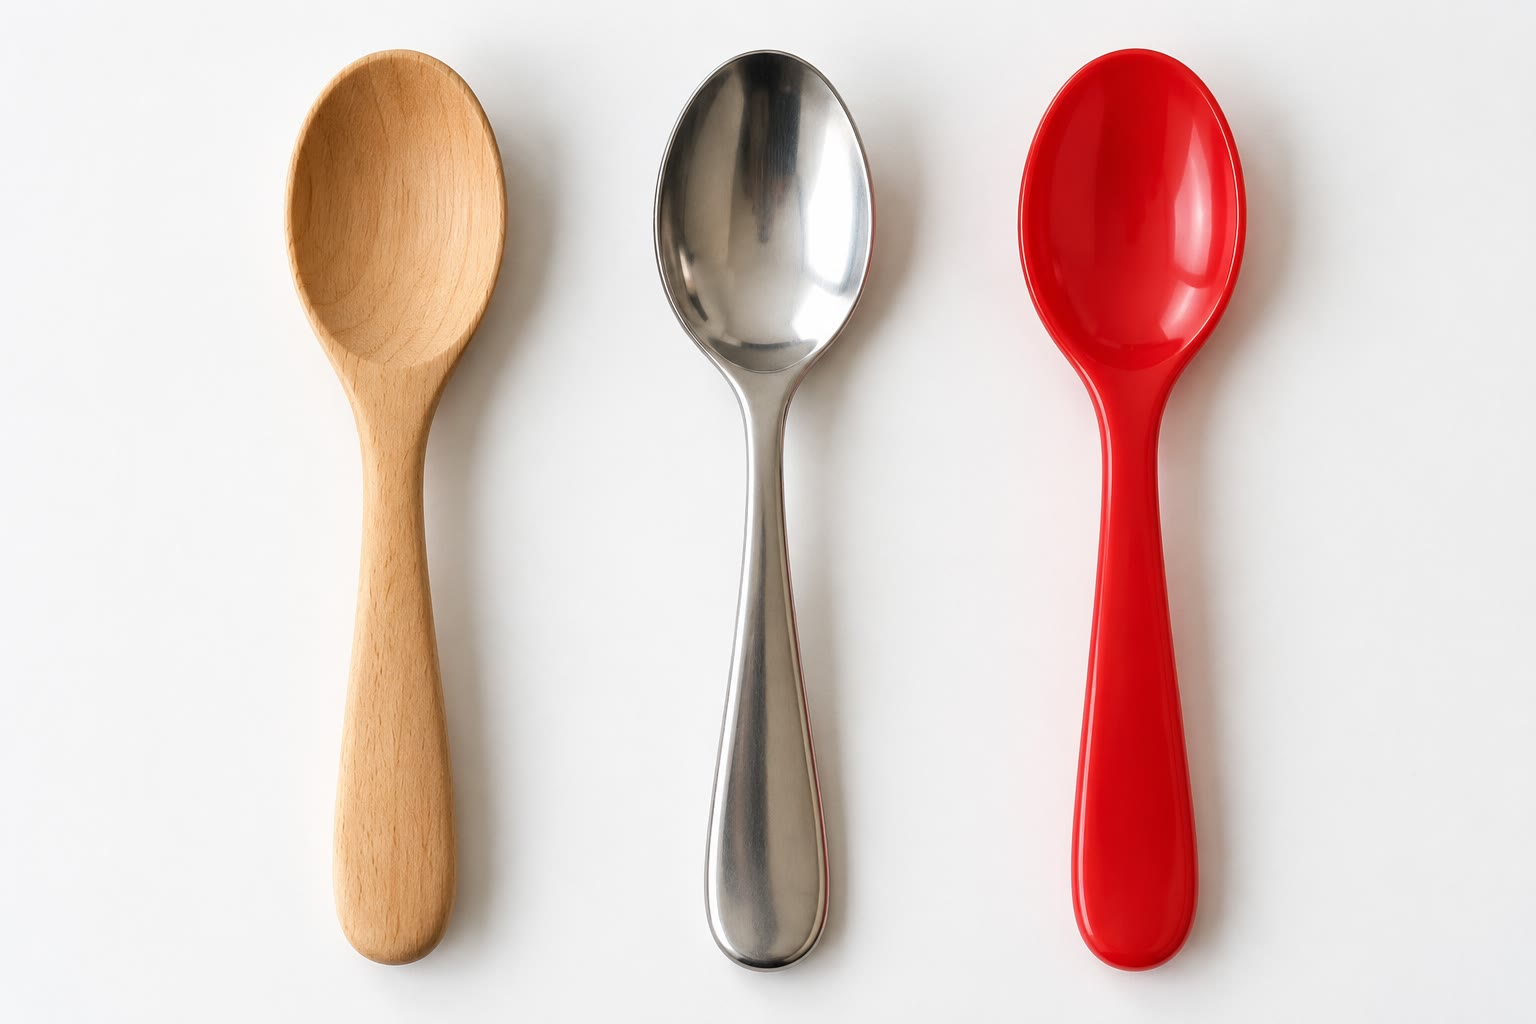
\includegraphics[width=0.55\linewidth]{images/book1/ai/g1-three-spoons.jpg}

{\small Três colheres: o mesmo \omterm{def:g1:materials-around-us:object}{objeto}, três materiais --- madeira, metal
e plástico.}
\end{omfigure}

\begin{example}[Um material, muitos objetos]\label{ex:g1:materials-around-us:wood}
A madeira é o \omterm{def:g1:materials-around-us:material}{material} de um lápis, de uma cadeira, de uma porta, de um
trenzinho de brinquedo e de uma colher de pau. Muitos \omterm{def:g1:materials-around-us:object}{objetos} diferentes
podem ser feitos do mesmo \omterm{def:g1:materials-around-us:material}{material}.
\end{example}

\begin{remark}[Objetos feitos de vários materiais]\label{rem:g1:materials-around-us:several}
Muitos \omterm{def:g1:materials-around-us:object}{objetos} são feitos de mais de um \omterm{def:g1:materials-around-us:material}{material}. Uma tesoura tem
lâminas de metal e cabo de plástico. Um lápis é de madeira por fora e
tem por dentro um bastãozinho cinza de grafite. Uma janela é de vidro
numa moldura de madeira, de metal ou de plástico.
\end{remark}

\section{Sete materiais comuns}

\begin{proposition}[Materiais por toda parte]\label{prop:g1:materials-around-us:seven}
A maioria dos \omterm{def:g1:materials-around-us:object}{objetos} à nossa volta é feita de poucos materiais comuns:
\begin{itemize}
  \item \textbf{madeira}: mesas, cadeiras, lápis, portas;
  \item \textbf{metal}: garfos, chaves, pregos, panelas, bicicletas;
  \item \textbf{vidro}: janelas, potes, garrafas, copos;
  \item \textbf{plástico}: tigelas, garrafas, brinquedos, baldes;
  \item \textbf{papel} e papelão: livros, guardanapos, caixas;
  \item \textbf{tecido}: roupas, cortinas, bolsas --- feitos de lã,
        de algodão ou de outros fios;
  \item \textbf{pedra}: muros, degraus, pedrinhas, estátuas.
\end{itemize}
\end{proposition}

\begin{omfigure}
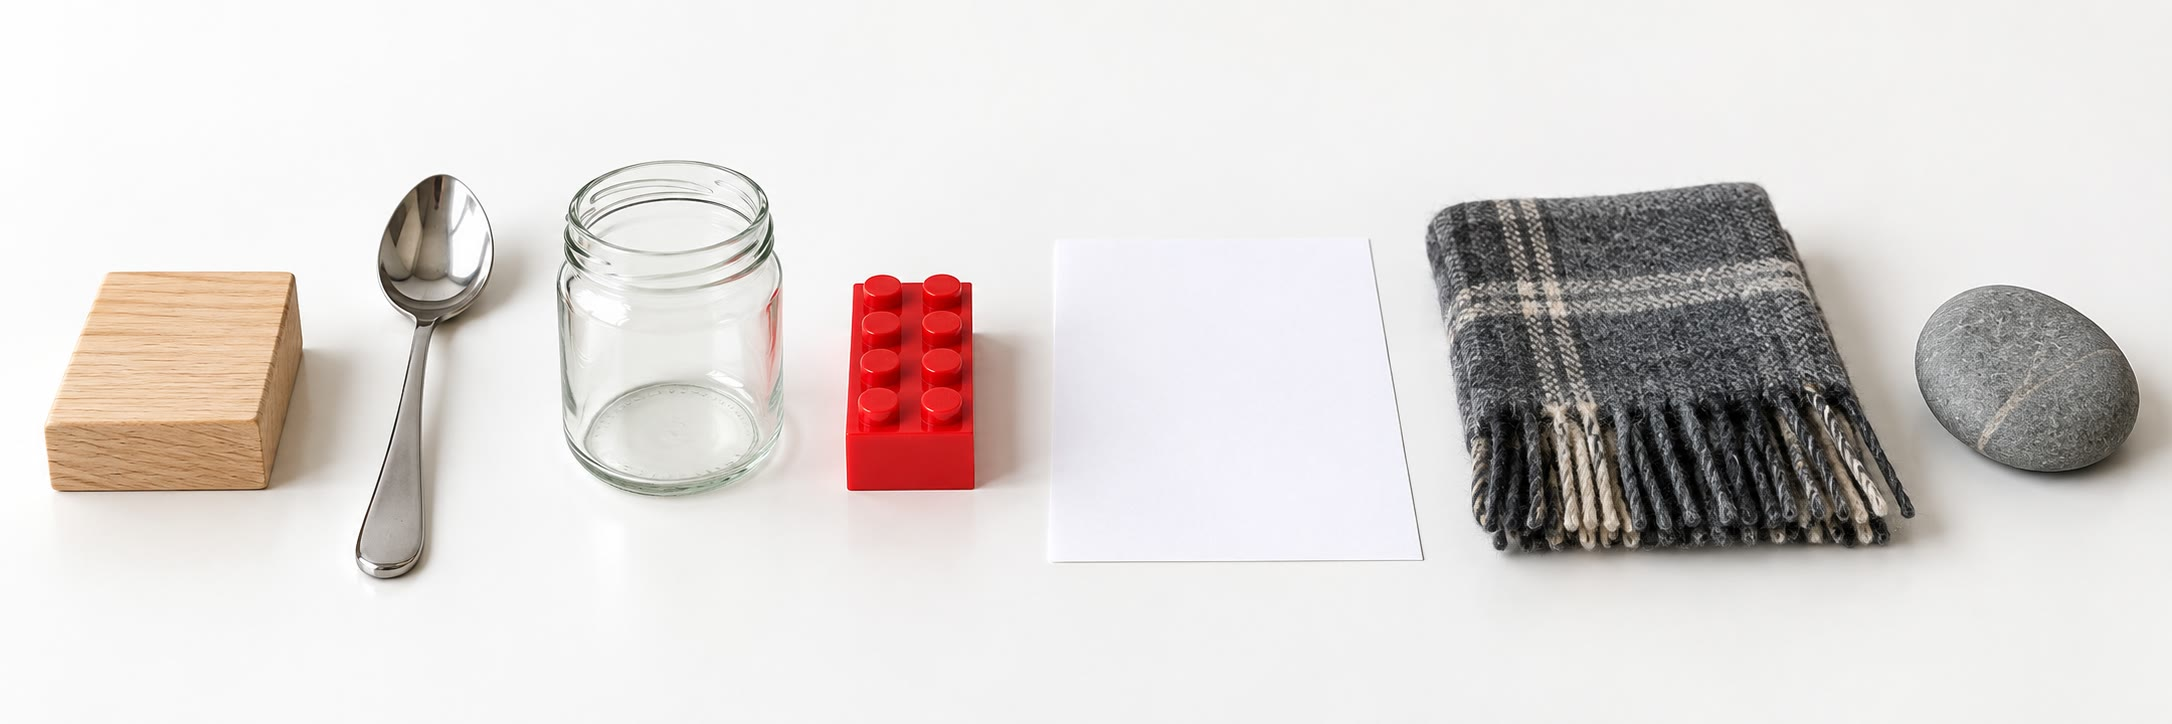
\includegraphics[width=0.75\linewidth]{images/book1/ai/g1-material-samples.jpg}

{\small Sete amostras, da esquerda para a direita: madeira, metal, vidro,
plástico, papel, tecido (lã) e pedra.}
\end{omfigure}

\begin{remark}[Nomes que também são materiais]\label{rem:g1:materials-around-us:names}
Chamamos o copo de ``copo'', mas ele é feito de vidro; já uma folha de
papel muitas vezes é chamada só de ``papel''. Aí a palavra do \omterm{def:g1:materials-around-us:object}{objeto} e
a palavra do \omterm{def:g1:materials-around-us:material}{material} são a mesma. Quando falamos de materiais, queremos
dizer a matéria de que a coisa é feita, não o \omterm{def:g1:materials-around-us:object}{objeto}.
\end{remark}

\section{Propriedades dos materiais}

\begin{definition}[Propriedade de um material]\label{def:g1:materials-around-us:property}
Uma \emph{propriedade de um material}\index{propriedade de um material} é
algo que podemos descobrir sobre ele olhando, tocando ou testando: ele é
duro ou macio? Dá para ver através dele? Um ímã o puxa? Ele flutua na
água ou afunda?
\end{definition}

\begin{example}[Duro e macio]\label{ex:g1:materials-around-us:hard}
Uma pedrinha é dura: apertá-la com o polegar não deixa marca. Um
cachecol de lã é macio: ele se dobra e se amassa na mão. A madeira, o
metal, o vidro e a pedra são duros; o tecido e o papel são macios e se
dobram com facilidade.
\end{example}

\begin{example}[Ver através]\label{ex:g1:materials-around-us:see-through}
Vemos o jardim através de uma janela: o vidro deixa a luz passar, e
dizemos que ele é \emph{transparente}. Não dá para ver através de uma
porta de madeira, de uma parede de tijolos ou de uma panela de metal.
Alguns plásticos são transparentes, como uma garrafa de água; outros não
são, como uma pecinha vermelha de montar.
\end{example}

\begin{example}[Atraído por um ímã]\label{ex:g1:materials-around-us:magnet}
Um ímã puxa para perto dele um clipe de aço, um prego de aço ou uma
chave de ferro. Ele não puxa a madeira, o vidro, o plástico, o papel, o
tecido nem a pedra. E, que surpresa, ele não puxa todos os metais: uma
latinha de alumínio e um fio de cobre ficam onde estão. Um ímã atrai os
\omterm{def:g1:materials-around-us:object}{objetos} de ferro e de aço, que é feito principalmente de ferro.
\end{example}

\begin{omfigure}
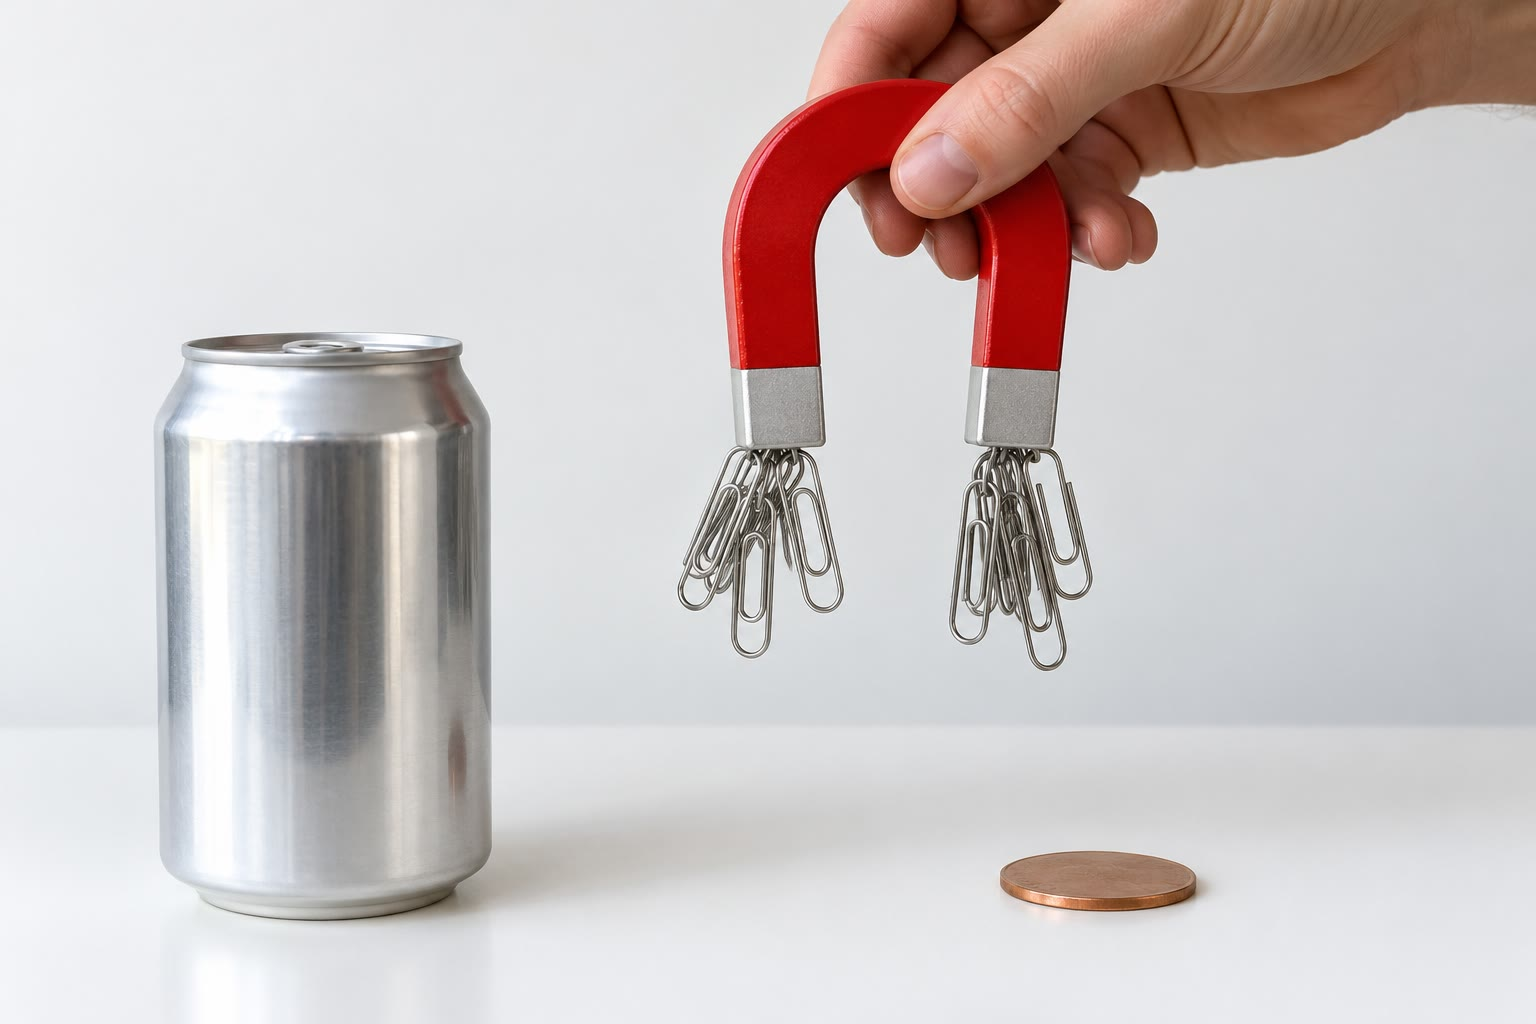
\includegraphics[width=0.55\linewidth]{images/book1/ai/g1-magnet-clips.jpg}

{\small Um ímã levanta clipes de aço. A latinha de alumínio e o disco de
cobre em cima da mesa ficam onde estão.}
\end{omfigure}

\begin{example}[Flutuar e afundar]\label{ex:g1:materials-around-us:float}
Ponha alguns \omterm{def:g1:materials-around-us:object}{objetos} numa bacia com água. Um bloco de madeira e uma
tampinha de garrafa de plástico flutuam. Uma pedrinha, uma bolinha de
gude de vidro e um prego de aço afundam até o fundo. Flutuar ou afundar
também é uma propriedade do \omterm{def:g1:materials-around-us:material}{material} da coisa.
\end{example}

\begin{omfigure}
\begin{tikzpicture}[font=\small]
  % the basin
  \fill[omWater!80] (0,0) rectangle (9,2.2);
  \draw[omGlass, line width=0.8pt] (-0.1,2.7) -- (0,2.6) -- (0,0) -- (9,0)
    -- (9,2.6) -- (9.1,2.7);
  % floating: wooden block, plastic cap
  \fill[brown!55, draw=brown!70!black] (0.8,2.0) rectangle (2.2,2.5);
  \fill[red!70, draw=red!50!black] (3.7,2.05) rectangle (4.3,2.35);
  % sunk: pebble, marble, nail
  \fill[black!35, draw=black!60] (5.0,0.25) ellipse (0.45 and 0.22);
  \shade[ball color=cyan!40] (6.5,0.2) circle (0.18);
  \fill[black!55] (7.6,0.06) rectangle (8.6,0.14);
  \fill[black!55] (7.52,0.02) rectangle (7.62,0.18);
  % labels
  \node[anchor=south] at (1.5,2.75) {madeira};
  \node[anchor=south] at (4.0,2.75) {tampinha};
  \node[anchor=north] at (5.0,-0.1) {pedrinha};
  \node[anchor=north] at (6.5,-0.1) {bolinha};
  \node[anchor=north] at (8.1,-0.1) {prego};
  \node[anchor=west, align=left] at (9.3,2.2) {estes flutuam};
  \node[anchor=west, align=left] at (9.3,0.2) {estes afundam};
\end{tikzpicture}

{\small Numa bacia com água: o bloco de madeira e a tampinha de plástico
flutuam; a pedrinha, a bolinha de gude de vidro e o prego de aço afundam.}
\end{omfigure}

\section{Separar os materiais}

\begin{method}[Separar por uma propriedade]\label{met:g1:materials-around-us:sort}
Para separar um monte de \omterm{def:g1:materials-around-us:object}{objetos}:
\begin{enumerate}
  \item escolha \textbf{uma} pergunta, por exemplo ``Um ímã puxa este
        \omterm{def:g1:materials-around-us:object}{objeto}?'';
  \item teste cada \omterm{def:g1:materials-around-us:object}{objeto} e ponha-o no grupo do ``sim'' ou no grupo do
        ``não'';
  \item depois, se quiser, separe cada grupo de novo com outra pergunta.
\end{enumerate}
Uma pergunta de cada vez: assim cada \omterm{def:g1:materials-around-us:object}{objeto} tem exatamente um lugar.
\end{method}

\begin{omfigure}
\begin{tikzpicture}[font=\small]
  \draw[omDef, line width=1pt] (0,0) circle (2.3);
  \draw[omProp, line width=1pt] (2.4,0) circle (2.3);
  \node[omDef, font=\small\bfseries] at (-0.6,2.65) {feito de metal};
  \node[omProp, font=\small\bfseries] at (3.0,2.65) {puxado por um ímã};
  \node[font=\footnotesize] at (-1.1,0.35) {latinha};
  \node[font=\footnotesize] at (-1.1,-0.35) {fio de cobre};
  \node[font=\footnotesize] at (1.2,0.6) {prego de aço};
  \node[font=\footnotesize] at (1.2,0) {chave de ferro};
  \node[font=\footnotesize] at (1.2,-0.6) {clipe};
  \node[font=\footnotesize] at (3.5,0) {(nada)};
  \node[anchor=west] at (5.2,0.9) {colher de pau};
  \node[anchor=west] at (5.2,0.3) {bolinha de gude};
  \node[anchor=west] at (5.2,-0.3) {cachecol de lã};
  \node[anchor=west] at (5.2,-0.9) {pedrinha};
\end{tikzpicture}

{\small Duas perguntas, dois aros. Dentro do aro azul: os \omterm{def:g1:materials-around-us:object}{objetos} feitos
de metal. Dentro do aro laranja: os \omterm{def:g1:materials-around-us:object}{objetos} que um ímã puxa. Nos dois
aros: os \omterm{def:g1:materials-around-us:object}{objetos} de ferro ou de aço. Fora dos dois: todo o resto.}
\end{omfigure}

\begin{center}
\small
\begin{tabular}{lccc}
\hline
\omterm{def:g1:materials-around-us:object}{objeto} (\omterm{def:g1:materials-around-us:material}{material}) & duro? & transparente? & puxado por um ímã? \\
\hline
bloco (madeira) & sim & não & não \\
prego (aço) & sim & não & sim \\
bolinha de gude (vidro) & sim & sim & não \\
tampinha (plástico) & sim & não & não \\
folha (papel) & não & não & não \\
cachecol (lã) & não & não & não \\
pedrinha (pedra) & sim & não & não \\
\hline
\end{tabular}
\end{center}

\section{O material certo para cada uso}

\begin{proposition}[Cada material é escolhido por suas propriedades]\label{prop:g1:materials-around-us:choose}
As pessoas escolhem o \omterm{def:g1:materials-around-us:material}{material} de um \omterm{def:g1:materials-around-us:object}{objeto} de acordo com o que o \omterm{def:g1:materials-around-us:object}{objeto}
precisa fazer:
\begin{itemize}
  \item uma janela precisa deixar a luz entrar: ela é feita de vidro,
        que é transparente;
  \item uma capa de chuva precisa segurar a chuva do lado de fora e
        poder ser dobrada: ela é feita de plástico ou de um tecido que a
        água não atravessa;
  \item uma panela não pode derreter no fogão: ela é feita de metal;
  \item o cabo de uma panela não pode queimar a mão: muitas vezes ele é
        feito de madeira ou de um plástico duro, que não esquentam tanto
        quanto o metal;
  \item um travesseiro precisa ser macio: ele é feito de tecido cheio
        de penas ou de fibras.
\end{itemize}
\end{proposition}

\begin{example}[Um barquinho]\label{ex:g1:materials-around-us:boat}
Um barquinho de brinquedo precisa flutuar. Ele pode ser feito de madeira
ou de plástico. Um barco feito de um bloco maciço de pedra afundaria na
hora.
\end{example}

\begin{remark}[Vidro quebrado]\label{rem:g1:materials-around-us:glass}
O vidro é duro, mas quebra, e os cacos cortam. Quando um copo quebra,
quem recolhe os cacos é um adulto.
\end{remark}

\section{Exercícios}

\begin{exercise}[$\star$]\label{exo:g1:materials-around-us:1}
Uma cadeira é um \omterm{def:g1:materials-around-us:object}{objeto} ou um \omterm{def:g1:materials-around-us:material}{material}? A madeira é um \omterm{def:g1:materials-around-us:object}{objeto} ou um
\omterm{def:g1:materials-around-us:material}{material}?
\end{exercise}

\begin{exercise}[$\star$]\label{exo:g1:materials-around-us:2}
Diga o \omterm{def:g1:materials-around-us:material}{material} de cada \omterm{def:g1:materials-around-us:object}{objeto}: o vidro de uma janela, um prego, uma
pedrinha, um livro, uma meia.
\end{exercise}

\begin{exercise}[$\star$]\label{exo:g1:materials-around-us:3}
Dê dois \omterm{def:g1:materials-around-us:object}{objetos} feitos de madeira e dois \omterm{def:g1:materials-around-us:object}{objetos} feitos de plástico.
\end{exercise}

\begin{exercise}[$\star$]\label{exo:g1:materials-around-us:4}
Descubra o intruso e diga por quê: uma colher de pau, um garfo de
metal, uma colher de plástico, uma cadeira de madeira. (Olhe os
materiais.)
\end{exercise}

\begin{exercise}[$\star$]\label{exo:g1:materials-around-us:5}
Através de qual \omterm{def:g1:materials-around-us:material}{material} dá para ver: a madeira, o vidro ou a pedra?
\end{exercise}

\begin{exercise}[$\star$]\label{exo:g1:materials-around-us:6}
Um ímã é aproximado de um prego de aço, de uma bolinha de gude de vidro
e de um bloco de madeira. Qual deles o ímã puxa?
\end{exercise}

\begin{exercise}[$\star$]\label{exo:g1:materials-around-us:7}
Olhe a figura da bacia. Quantos \omterm{def:g1:materials-around-us:object}{objetos} flutuam? Quantos afundam?
\end{exercise}

\begin{exercise}[$\star$]\label{exo:g1:materials-around-us:8}
Uma tesoura tem lâminas e cabo. De que \omterm{def:g1:materials-around-us:material}{material} é feita cada parte?
A tesoura é feita de um \omterm{def:g1:materials-around-us:material}{material} só ou de dois?
\end{exercise}

\begin{exercise}[$\star$]\label{exo:g1:materials-around-us:9}
Olhe a figura dos dois aros. Em que aro está a latinha? Por que ela não
está no aro laranja?
\end{exercise}

\begin{exercise}[$\star\star$]\label{exo:g1:materials-around-us:10}
Por que as janelas são feitas de vidro e não de madeira?
\end{exercise}

\begin{exercise}[$\star\star$]\label{exo:g1:materials-around-us:11}
O Sam quer separar estes 8 \omterm{def:g1:materials-around-us:object}{objetos} com a pergunta ``Um ímã puxa este
\omterm{def:g1:materials-around-us:object}{objeto}?'': um prego de aço, um clipe, uma pedrinha, uma colher de pau,
uma chave de ferro, uma latinha, uma bolinha de gude de vidro, uma meia
de lã. Quantos \omterm{def:g1:materials-around-us:object}{objetos} vão para o grupo do ``sim''? E quantos para o
grupo do ``não''?
\end{exercise}